\documentclass[border=3pt]{standalone}
\usepackage{tikz}
\usetikzlibrary{arrows.meta,calc,positioning}
\tikzset{st/.style={draw, thick, circle, minimum size=13mm, font=\sffamily\bfseries},
  pin/.style={-{Stealth[length=5pt]}, thick},
  lab/.style={font=\sffamily\footnotesize, align=center}}
\begin{document}
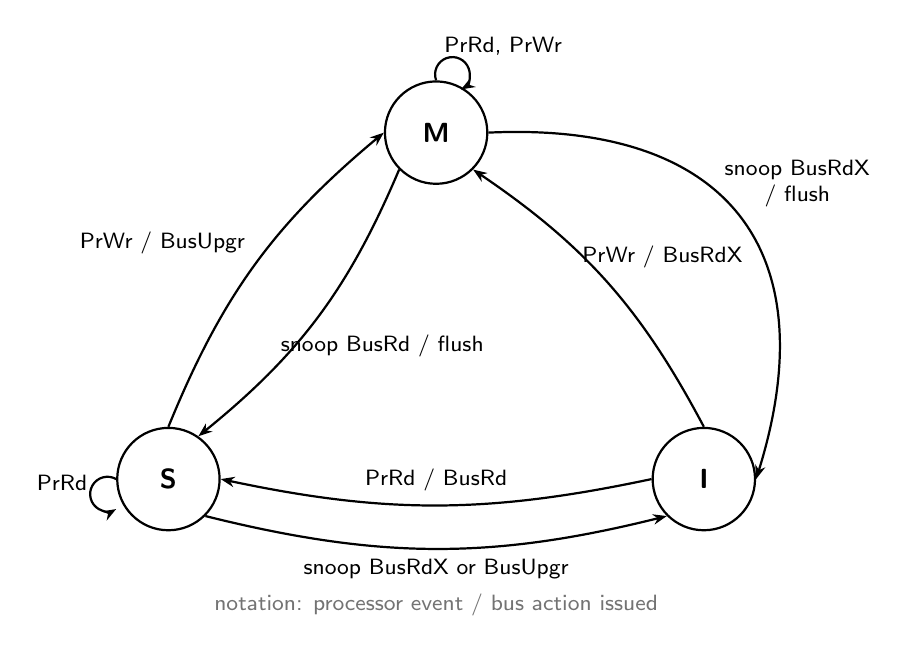
\begin{tikzpicture}[font=\sffamily\small]
  \node[st] (m) at (0,4.4)   {M};
  \node[st] (s) at (-3.4,0)  {S};
  \node[st] (i) at (3.4,0)   {I};
  % I -> S : processor read
  \draw[pin] (i.west) to[bend left=12] node[lab, above=0.5mm]{PrRd / BusRd} (s.east);
  % S -> M : processor write
  \draw[pin] (s.north) to[bend left=14] node[lab, above left=0mm and 0mm]{PrWr / BusUpgr} (m.west);
  % I -> M : processor write
  \draw[pin] (i.north) to[bend right=14] node[lab, pos=0.55, above right=-1mm and -3mm]{PrWr / BusRdX} (m.south east);
  % M -> S : observed BusRd, supply data
  \draw[pin] (m.south west) to[bend left=14] node[lab, below right=1mm and -6mm]{snoop BusRd / flush} (s.55);
  % M -> I : observed BusRdX
  \draw[pin] (m.east) to[bend left=55, looseness=1.4] node[lab, pos=0.4, right=1mm]{snoop BusRdX\\/ flush} (i.east);
  % S -> I : observed BusRdX/BusUpgr
  \draw[pin] (s.south east) to[bend right=14] node[lab, below]{snoop BusRdX or BusUpgr} (i.south west);
  % self loops
  \draw[pin] (m.north) arc (200:-60:2.2mm) ;
  \node[lab] at (0.85,5.5) {PrRd, PrWr};
  \draw[pin] (s.west) arc (60:300:2.2mm);
  \node[lab] at (-4.75,-0.05) {PrRd};
  \node[lab, text=black!55] at (0,-1.6) {notation: processor event / bus action issued};
\end{tikzpicture}
\end{document}
